  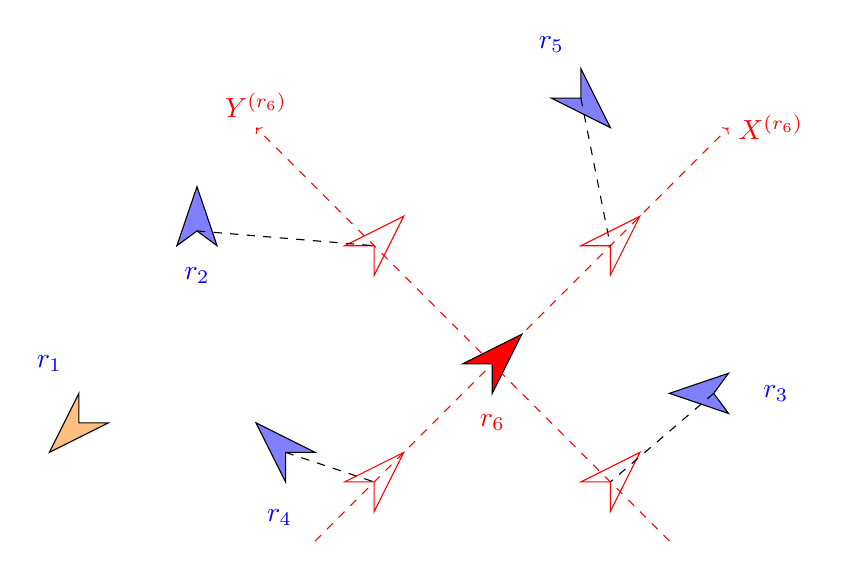
\begin{tikzpicture}[scale=1.5]
    \draw[fill=red] (3,3) -- (2.75,3) -- (3.25,3.25) -- (3,2.75)        -- cycle;
    \node[color=red] at (3, 2.5) {$r_6$};
    %\draw[thick, ->] (-1,0) -- (6,0) node[right] {X};
    %\draw[thick, ->] (0,-1) -- (0,6) node[above] {Y};
    \draw[color=red, dashed, ->] (1.5,1.5) -- (5,5) node[right] {$X^{(r_6)}$};
    \draw[color=red, dashed, ->] (4.5,1.5) -- (1,5) node[above] {$Y^{(r_6)}$};
    % draw grids
    %\draw[color=gray, help lines, line width=.05pt] (-1,1)  grid[xstep=.5cm, ystep=.5cm] (6,6);
    \draw[fill=blue!50] (0.5,4.5) -- (0.33,4) -- (0.5,4.125) -- (0.67,4)    -- cycle;
    \node[color=blue] at (0.5,3.75) {$r_2$};
    \draw[fill=blue!50] (4,5) -- (3.75,5.5) -- (3.75,5.25) -- (3.5,5.25)        -- cycle;
    \node[color=blue] at (3.5,5.7) {$r_5$};
    \draw[fill=blue!50] (1,2.5) -- (1.25,2) -- (1.25,2.25) -- (1.5,2.25)        -- cycle;
    \node[color=blue] at (1.2,1.7) {$r_4$};
    \draw[fill=blue!50] (5,2.92) -- (4.5,2.75) -- (5,2.58) -- (4.875,2.75)  -- cycle;
    \node[color=blue] at (5.4,2.75) {$r_3$};
%    \draw[fill=blue!50] (2.5,0) -- (2.7,0.52) -- (2.5,0.35) -- (2.3,0.52)   -- cycle;
%    \node[color=blue] at (2.5,0.75) {$r_1$};
    \draw[fill=orange!50] (-0.5,2.5) -- (-0.5,2.75) -- (-0.75,2.25) -- (-0.25,2.5)  -- cycle;
    \node[color=blue] at (-0.75,3) {$r_1$};
        
    \draw[color=red] (4,4) -- (3.75,4) -- (4.25,4.25) -- (4,3.75) -- cycle;
    \draw[color=red] (2,2) -- (1.75,2) -- (2.25,2.25) -- (2,1.75) -- cycle;
    \draw[color=red] (2,4) -- (1.75,4) -- (2.25,4.25) -- (2,3.75) -- cycle;
    \draw[color=red] (4,2) -- (3.75,2) -- (4.25,2.25) -- (4,1.75) -- cycle;
        
    \draw[dashed](0.5, 4.125) -- (2,4);
    \draw[dashed](1.25,2.25) -- (2,2);
    \draw[dashed](3.75,5.25) -- (4,4);
    \draw[dashed](4.875,2.75) -- (4,2);
%   \draw (0,-4.75) node[below] {reflect across $x$-axis};  
  \end{tikzpicture}